\label{chapter:ModelExecution} 

The steps in the model execution workflow are:
\begin{enumerate}
    \item Run Modflow to create the new project output files (e.g.\ time-varying hydraulic head, drawdown etc).\label{step:modflow}
    \item Run \verb+_post.mut+ to post-process the Modflow project, which produces \tecplot\ output files for the various Modflow domains (i.e.\ \gwf,\swf\ and/or \cln ) created during the Modflow simulation.\label{step:mut2}
    \item Run \tecplot\ and examine the Modflow output files.   \label{step:Tecplot2}
\end{enumerate}
In this tutorial, we will build a 3D fully-coupled \gwf -SWF model, check the build using \tecplot, run \mfus\ to generate output, then examine the results using \tecplot.

\begin{verbatim}
    ! This example builds a modflow project of the Abdul Field Experiment
    ! The\swf\ mesh and top of the\gwf\ mesh are defined by a 2D Grid Builder triangular mesh
    build modflow usg
\end{verbatim}

Any input line beginning with  is considered to be a comment and will be ignored by \mut\.  Here we begin the file with two comments describing the project.

The third line activates the \mut\ 'build modflow usg' environment, which accepts further instructions required to define the project. This environment can be split into roughly 4 sections:
\begin{description}
    \item[Grid definition] Instructions for defining the \gwf,\swf\ and\cln\ numerical discretizations.
    \item[Modflow parameters] Instructions for supplying Modflow parameter values (e.g. solver inputs for the SMS package, hydraulic properties for the LPF package etc.)
    \item[Stress periods, boundary conditions] These instructions are repeated once for each desired stress period and include instructions about time stepping parameters and boundary conditions that are to be applied.
    \item[Output control] Instructions defining a list of output times at which Modflow output files (e.g. heads, drawdowns, cell-by-cell flows etc.) are to be written.
\end{description}


The first group of instructions are used to build the Modflow unstructured mesh. \mut\ requires a 2D 'template'

\begin{verbatim}
    ! -----------------------------------Grid definition
    2d mesh from gb
    ./gb/grid
\end{verbatim}

\section*{Step~\ref{step:copy}: Copy an Existing \mut\ Project}

Create a new folder called e.g. \verb+My_Project+ and copy the folder \verb+MUT_Examples\6_Abdul_Prism_Cell+ into it.
Figure~\ref{fig:my_project} shows the contents of our \verb+6_Abdul_Prism_Cell+ folder.  Yours may look different depending on the root drive and folder location.
\begin{figure}[h!]
    \centering
    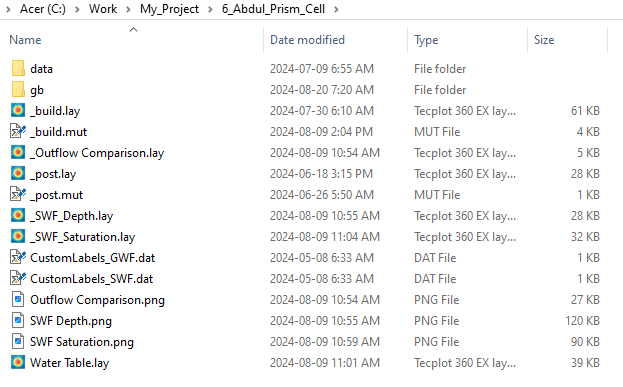
\includegraphics[width=0.8\textwidth]{abdul_folder_contents}
    \caption{The contents of the 6\_Abdul\_Prism\_Cell folder}
    \label{fig:my_project}
\end{figure}

This example contains several files you might typically find in a \mut\ Modflow project, including \mut\ input files (extension .mut), \tecplot\ layout files (extension .lay), \tecplot\ input files (extension .dat).  For now, our focus will be on the \mut\ input file \_\verb+build.mut+.

\section*{Step~\ref{step:modify}: Modify the Input File(s)}
The input file \_\verb+build.mut+ is set up to build a Modflow project.  If you open the file in a text editor you will see that it consists of a sequence of comments (lines beginning with an exclamation mark \verb+!+), \mut\ instructions and data (numbers or alphanumeric strings).  Details of the input file contents are described in detail in Section~\ref{InputFileDetails}.  For now, we will only make a minor change to the input file before moving on to the next step, which is to add a new comment line of your choice at the start of the file.

\section*{Step~\ref{step:mut1}: Execute \mut\ to Build the Project}


Assuming you have followed the set-up instructions in Section~\ref{Install}, you can execute \mut\ with the input file \_\verb+build.mut+ by typing:
\begin{verbatim}
    mut _build
\end{verbatim}




\section*{Step~\ref{step:modflow}: Run Modflow to Generate Output}
\section*{Step~\ref{step:mut2}: Run \mut\ to Post-Process the Modflow Output}
\section*{Step~\ref{step:Tecplot2}: Run \tecplot\ to Visualize the Modflow Output}

